% Generated from tex/chapters/ch04/00_chapter_opening.tex, tex/chapters/ch04/01_全体概要：この章で学ぶこと.tex, tex/chapters/ch04/02_最初に必要な用語.tex, tex/chapters/ch04/03_略語.tex, and tex/chapters/ch04/04_導入：ソフトウェア構築とは何か.tex for the SWEBOK structure tree
\section{第04章 ソフトウェア構築}
\noindent\textbf{この資料の主張}

ソフトウェア構築は、単にプログラムを書く作業ではない。要求と設計を、実行でき、検証でき、保守できるソフトウェアへ変える中心的な活動である。構築には、コーディング、検証、単体テスト、統合テスト、デバッグ、再利用、統合、依存関係管理、性能調整、開発環境の選択が含まれる。よい構築は、複雑さを抑え、変化を受け入れ、欠陥を早く見つけ、既存資産を適切に使い、標準に沿って進めることで実現する。

\begin{plainbox}
\textbf{この資料の読み方}

専門用語は原則として日本語で示し、必要に応じて英語を括弧内に併記する。英語名は、元資料やツール上の名称を確認したいときの手がかりとして残す。初学者が前提知識なしに読めるように、各節では「何のための概念か」「実務では何を見ればよいか」を重視する。
\end{plainbox}

\subsection*{全体概要：この章で学ぶこと}
\addcontentsline{toc}{subsection}{全体概要：この章で学ぶこと}

この章は、ソフトウェアを実際に作る段階で必要になる知識を扱う。ここでいう「作る」とは、ソースコードを書くことだけではない。詳細設計を補い、テストし、部品を統合し、依存関係を管理し、性能を測り、運用に近い環境からのフィードバックを得ながら、ソフトウェアを完成度の高い形に近づけることである。

\noindent\textbf{到達目標}\quad この章を読み終えると、次のことができるようになる。

\begin{itemize}
  \item ソフトウェア構築が、設計、テスト、品質、構成管理、プロジェクト管理とどう関係するかを説明できる。
  \item 複雑さの最小化、変化への備え、検証しやすさ、再利用、標準適用の意味を説明できる。
  \item コーディング、単体テスト、統合、依存関係管理、継続的統合の実務上の役割を説明できる。
  \item API、例外処理、実行可能モデル、状態機械、ミドルウェア、クラウド、並行処理、性能調整などの構築技術を概観できる。
  \item 開発環境、単体テストツール、性能分析ツール、ローコード/ゼロコード環境の位置づけを説明できる。
\end{itemize}

\noindent\textbf{学習順序}\quad 初学者は、まず「構築とは何か」と「構築の基本原則」を押さえる。その後、「構築をどう管理するか」「現場で何を考えるか」「どの技術を使うか」「どのツールが支えるか」という順で読むとよい。

\begin{figure}[htbp]
\centering
\IfFileExists{assets/generated_figures/ch04/fig-ch04-01.png}{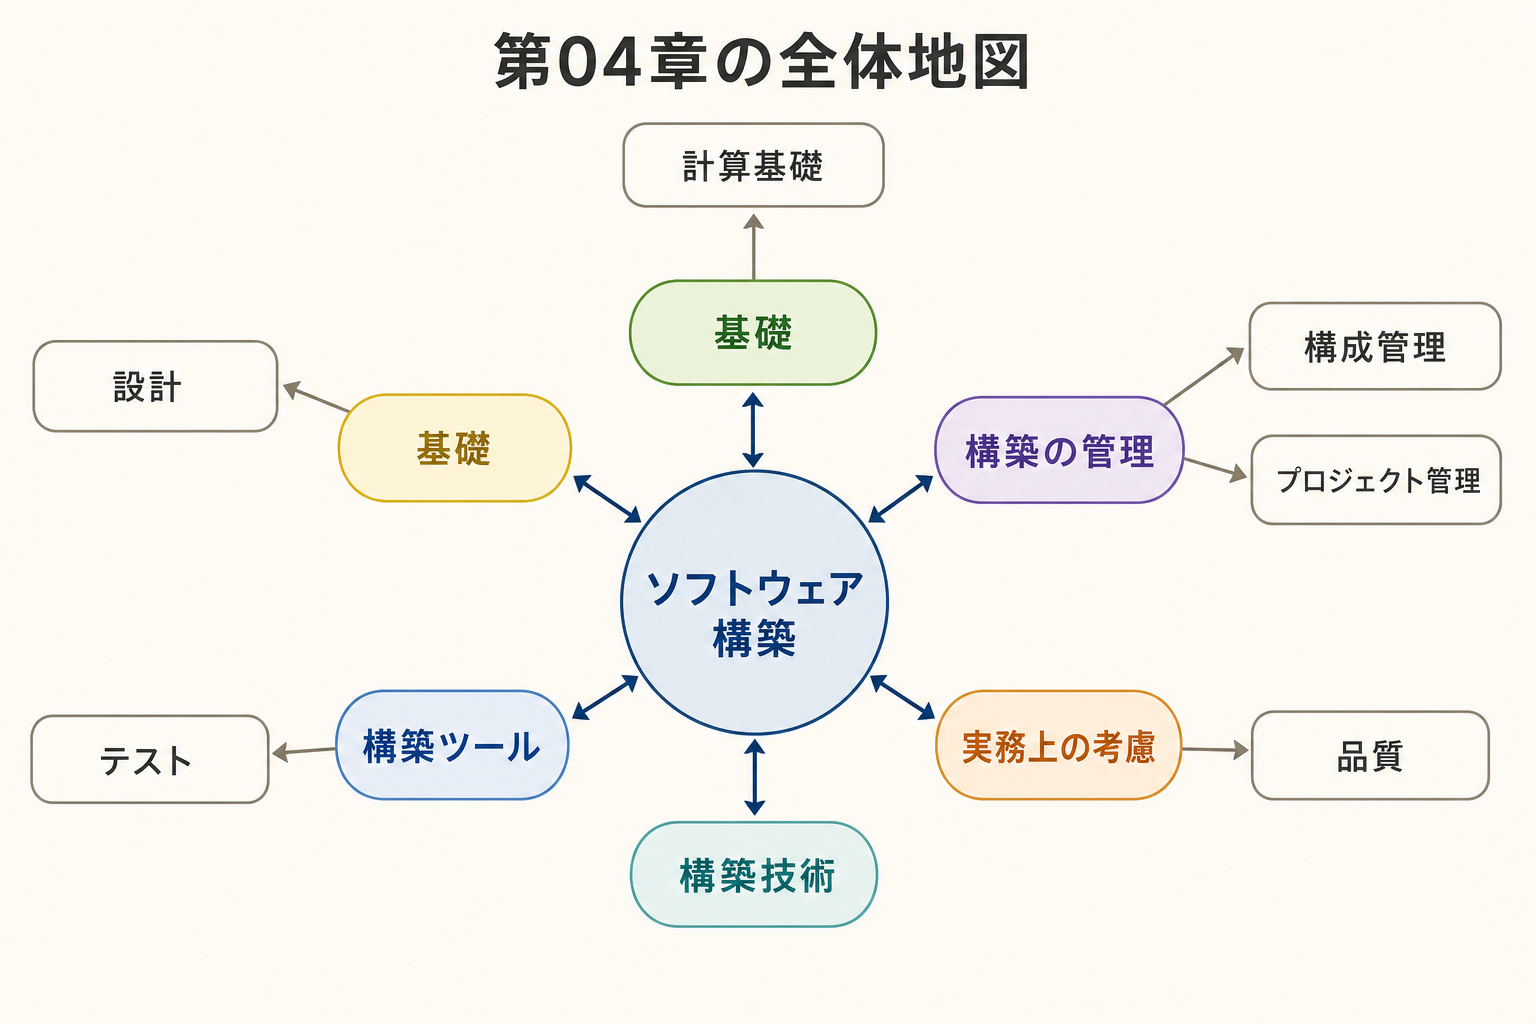
\includegraphics[width=0.96\linewidth]{assets/generated_figures/ch04/fig-ch04-01.png}}{\fbox{\parbox[c][48mm][c]{0.9\linewidth}{\centering 画像生成待ち\\第04章の全体地図}}}
\caption{第04章の全体地図}
\label{fig:ch04-01}
\end{figure}

\subsection*{最初に必要な用語}
\addcontentsline{toc}{subsection}{最初に必要な用語}

\par\smallskip\noindent\refstepcounter{table}\label{tab:ch04-01}\textbf{表 \thetable: 第04章 ソフトウェア構築 表01}\par\smallskip
\begin{longtable}{L{0.23\linewidth}L{0.69\linewidth}}
\toprule
\textbf{用語} & \textbf{初学者向けの説明} \\
\midrule
ソフトウェア構築 & ソフトウェアを詳細に作成・保守する活動である。コーディング、検証、単体テスト、統合テスト、デバッグなどを含む。 \\
コーディング & プログラミング言語などを使い、設計や要求を実行可能な形に書き表すこと。 \\
検証 & 作ったものが、仕様、設計、標準、期待された振る舞いを満たしているか確認すること。 \\
単体テスト & クラス、関数、モジュールなど、個別の部品を単独で確認するテスト。 \\
統合テスト & 複数の部品を組み合わせたとき、相互作用が正しく働くかを確認するテスト。 \\
デバッグ & 失敗の原因となる欠陥を見つけ、原因を理解し、修正する作業。 \\
依存関係 & 自分のソフトウェアが利用する外部ライブラリ、フレームワーク、部品、サービスなどとの関係。 \\
継続的統合 & 変更を頻繁に統合し、自動ビルドと自動テストで早く問題を発見する実践。 \\
再利用 & 既存の部品、コード、ライブラリ、サービス、設計パターンなどを別の問題解決に使うこと。 \\
API & アプリケーションプログラミングインタフェースのことである。ライブラリやサービスを利用するために公開された操作、引数、意味の取り決めである。 \\
\bottomrule
\end{longtable}

\subsection*{略語}
\addcontentsline{toc}{subsection}{略語}

\par\smallskip\noindent\refstepcounter{table}\label{tab:ch04-02}\textbf{表 \thetable: 第04章 ソフトウェア構築 表02}\par\smallskip
\begin{longtable}{L{0.16\linewidth}L{0.32\linewidth}L{0.44\linewidth}}
\toprule
\textbf{略語} & \textbf{日本語} & \textbf{説明} \\
\midrule
API & アプリケーションプログラミングインタフェース & ライブラリ、サービス、フレームワークを使うための公開された入り口。 \\
CI & 継続的統合 & 変更を頻繁に統合し、自動ビルドと自動テストで確認する実践。 \\
COTS & 商用既製品 & 自作ではなく、市販または既存の製品として利用するソフトウェア部品。 \\
DSL & ドメイン固有言語 & 特定領域の問題を表しやすいように作られた言語。 \\
IDE & 統合開発環境 & 編集、ビルド、テスト、デバッグなどを統合した開発環境。 \\
MDA & モデル駆動アーキテクチャ & モデルから実装へ変換する考え方を中心にした開発方式。 \\
PIM & プラットフォーム非依存モデル & 特定の実装環境に依存しない解決策のモデル。 \\
PSM & プラットフォーム固有モデル & 実装環境の詳細を含むモデル。 \\
TDD & テスト駆動開発 & テストを先に書き、そのテストを通すようにコードを書く開発スタイル。 \\
WYSIWYG & 見たままが得られる方式 & 画面上の見た目が成果物の見た目に近い編集方式。 \\
\bottomrule
\end{longtable}

\subsection*{導入：ソフトウェア構築とは何か}
\addcontentsline{toc}{subsection}{導入：ソフトウェア構築とは何か}

ソフトウェア構築とは、ソフトウェアを詳細に作成し、保守する活動である。具体的には、コーディング、検証、単体テスト、統合テスト、デバッグを含む。構築は、設計書の内容をただ機械的に写す作業ではない。多くの現場では、詳細な設計判断の一部が構築中に行われる。たとえば、どのデータ構造を使うか、エラーをどこで検出するか、処理をどの関数に分けるか、どのライブラリを使うかは、構築段階で決まることが多い。

この章の知識領域は、他の知識領域と強く結びつく。設計の成果物を入力として使い、テストに渡す成果物を作るため、ソフトウェア設計とソフトウェアテストとの関係が特に強い。また、構築ではソースファイル、テストケース、設定ファイル、文書など多数の構成品目が生まれるため、ソフトウェア構成管理とも密接に関係する。品質、プロジェクト管理、計算基礎とも関係が深い。

\begin{keybox}{重要}
ソフトウェア構築は、実装だけでなく「実装を検証可能にし、変更可能にし、統合可能にし、保守可能にする活動」である。したがって、構築の品質は、完成したソフトウェアの品質だけでなく、後続の変更や運用のしやすさにも影響する。
\end{keybox}

\begin{figure}[htbp]
\centering
\IfFileExists{assets/generated_figures/ch04/fig-ch04-02.png}{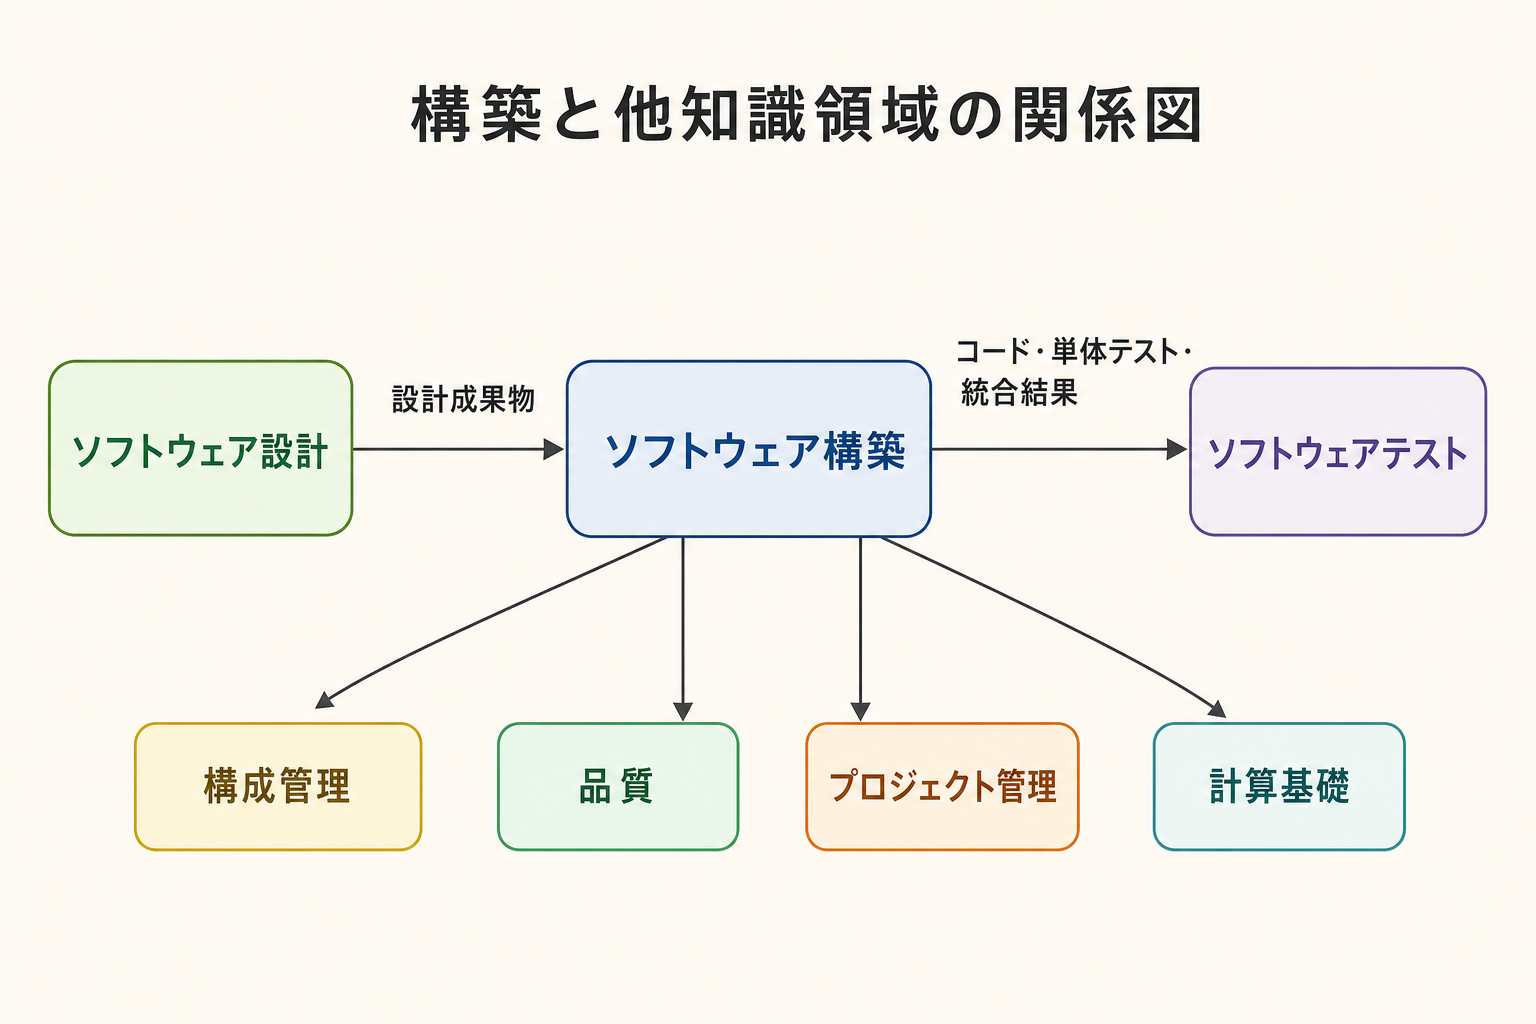
\includegraphics[width=0.96\linewidth]{assets/generated_figures/ch04/fig-ch04-02.png}}{\fbox{\parbox[c][48mm][c]{0.9\linewidth}{\centering 画像生成待ち\\構築と他知識領域の関係図}}}
\caption{構築と他知識領域の関係図}
\label{fig:ch04-02}
\end{figure}
